%\newcommand{\nsubparagraph}[1]{\textbf{#1}}
\newcommand{\AVG}{\mathit{AVG}}

\section{Empirical Evaluation}\label{sec:empiricalEvaluation}
In this section we discuss our analysis of the six strategies in terms of their runtime and accuracy response to typical errors that may occur when capturing an image of the sky.
For our testing, the astronomical catalog used to populate all relations in the reference database was the Hipparcos Input Catalogue~\cite{perryman:hipparcosCatalogue}. 
The $\texttt{REF}$ relation was shrunk to $1{,}471$ elements dependent on each star's brightness ($m < 4.5$) to reduce the size of the $\texttt{REF}_\texttt{STRATEGY}$ relations (and consequently the running time) for each strategy.
All simulations were performed $2{,}000$ times on a Raspberry Pi Model 3B+, implemented in C++14 without optimization, and utilized SQLite as the embedded SQL database engine.
%All queries involve the execution of a single \texttt{SELECT} statement on this file for each candidate retrieval step, with the exception of the Pyramid method which requires three.
Image data was generated as points randomly (but uniformly) rotated from the database coordinate system to remove the discrepancies that may arise from the image processing component.
Three types of errors were introduced to the image data from here: false positives, false negatives, and points whose position is misrepresented from the database (i.e.\ Gaussian noise).
The width of each strategy's range search was determined using a grid search, exploring boundaries from \num{1e-1}, \num{1e-2}, \ldots, to \num{1e-10}.
The exact implementation is available at the following link: \url{https://github.com/glennga/hoku}.

In a clean image (introducing no errors), all strategies are always able to produce a correct mapping from some image subset to the \texttt{REF} table.
The Pyramid and Interior Angle strategies are the fastest methods here ($6.293{\pm}0.167\si{ms}$), followed by the Angle strategy (81.249\si{ms}), with all methods possessing triangular features last ($122.479{\pm}1.940\si{ms}$).
Both the Pyramid and Interior Angle strategies do not utilize an optimal map determination procedure, which significantly reduces their runtime.
The Angle strategy, though still dependent on the direct-match test, has the smallest $\texttt{REF}_\texttt{STRATEGY}$ relation (2-combinations vs.\ 3-combinations) resulting in a slight speedup from the triangular featured strategies.

%The Interior Angle strategy is the fastest of all six, a factor of 3.5 times quicker than the next fastest method: the Pyramid strategy ($0.199\si{ms}$ vs.\ $0.710\si{ms}$).
%This is a direct result of utilizing extra storage to store the map in the Interior Angle strategy, avoiding the need to search the \texttt{REF} relation to determine an optimal map.
%The Pyramid and Composite Pyramid are additionally restricted by their voting-based verification steps, both of which require three additional database searches.

In an image of three to six false positives, the unmodified methods that perform the most accurately are the Angle, Planar Triangle, and Spherical Triangle strategies.
The source of error for all other methods are a result of exhausting all $b$ sets, as opposed to returning an incorrect map.
Removing the voting based confidence check eliminated this error for both the Pyramid and Composite Pyramid strategies, raising both accuracies to near 100\% with a runtime faster than the Angle, Planar Triangle, and Spherical Triangle strategies.
This difference in speed also demonstrates the efficacy of the pyramid $b$ decision in contrast to the naive approaches.
For the Interior Angle strategy, replacing its non exhaustive image subset decision with an exhaustive naive approach increased its accuracy to the near 100\%.
When dealing with this type of noise, not exploring all possible combinations increases the chance that a trio without false positives is never handled, thus lowering overall accuracy.
~\autoref{figure:results} depicts the accuracy of each strategy in its most optimal configuration under varying types of noise.

In an image of one to three light blocking blobs (resulting in false negatives), all strategies except the unaltered pyramid strategies perform with similar accuracy and runtime.
These errors stem as a result of an image possessing too few points to perform identification altogether.
The unaltered pyramid strategies require a minimum of four points, raising the chance of having too little stars to perform identification and decreasing the overall accuracy.
Removing the verification step for the pyramid methods raises the Composite Pyramid accuracy to a similar range of the rest and does not significantly affect the Pyramid accuracy, suggesting that this verification step is too aggressive of a filter overall.
In terms of speed the Interior Angle method is the fastest of the six, followed closely by Pyramid method ($5.791\si{ms}$ vs.\ $6.050\si{ms}$).

In an image with Gaussian noise of $\sigma \seq 0.0001^\circ$ to $\sigma \seq 0.0002^\circ$, the Angle strategy is the most accurate but runs nearly 15 times as long as the 2nd most accurate \& fastest overall strategy: the Pyramid strategy without a verification step ($208.552\si{ms}$ vs.\ $13.801\si{ms}$).
Unlike the results of the previous simulations, we now see incorrect maps returned by strategies instead of returning with an error.
Though small, these maps are only produced by the strategies with triangular features (Planar Triangle, Spherical Triangle, Composite Pyramid).
Interstar angles appear to be the most effective feature set against Gaussian noise.

\section{Conclusion}\label{sec:conclusion}
To conclude, the Angle strategy is the most accurate strategy under all types of noise, but is the slowest of the six.
The Pyramid strategy without a verification step is the next best strategy in terms of accuracy, and is the fastest overall method.
The Interior Angle strategy was improved by using a naive image subset decision and has the lowest floor in terms of speed, however this strategy handles Gaussian noise the worst of the six. 
The triangular strategies lie between the Angle and Interior Angle methods in terms of accuracy, but are a faster alternative to the Angle method.
The Composite Pyramid strategy attempts to utilize a different feature set with the effectiveness of the Pyramid core but ultimately inherits the worst of each strategy.

\begin{figure}
    \centering{
    \begin{tikzpicture}
    \begin{axis}[
    ybar,
    width=\linewidth, height=5cm,
    ylabel={Accuracy of Map}, ylabel near ticks, ymin=0.5, ymax=1.25,
    ytick={0.6, 0.8, 1},
    xtick={1, 2, 3}, xticklabels={False Positives, False Negatives, Gaussian Noise},
    xmin=0.5, xmax=3.5, xtick pos=left,
    nodes near coords, every node near coord/.append style={rotate=90, anchor=west},
    legend style={at={(0.5,-0.25)}, anchor=north,legend columns=-1},
    bar width=7,
    every node near coord/.append style={
    	/pgf/number format/fixed zerofill,
    	/pgf/number format/precision=4
	}
    ]
        \addplot coordinates {(1, 1.0) (2, 0.9955) (3, 0.8825)};
        \addplot coordinates {(1, 0.9975) (2, 0.97025) (3, 0.5245)};
        \addplot coordinates {(1, 0.983083333333333) (2, 0.99625) (3, 0.697916666666667)};
        \addplot coordinates {(1, 0.9905) (2, 0.9965) (3, 0.701666666666667)};
        \addplot coordinates {(1, 1.0) (2, 0.973) (3, 0.82025)};
        \addplot coordinates {(1, 0.99875) (2, 0.972) (3, 0.579416666666667)};
        \legend{ANG, INT, SPH, PLN, PYR, COM}
    \end{axis}
\end{tikzpicture}

%\begin{tikzpicture}
%	\begin{axis}[width=\linewidth, height=5cm,
%				symbolic x coords={ANG,INT,SPH,PLN,PYR,COM},
%				xtick=data,bar width=20, ybar, colorbar,
%				]
%\addplot+[point meta=explicit, scatter] table[x=IDE,y=ACC,meta=SPE,col sep=semicolon]{
%	IDE;ACC;SPE
%	ANG;0.95954045954046;22.3882783882784
%	INT;0.827922077922078;2.48135198135198
%	SPH;0.887667887667888;18.7967032967033
%	PLN;0.901986901986902;17.5726773226773
%	PYR;0.931401931401931;1.08050283050283
%	COM;0.855033855033855;8.25524475524475
%};
%	\end{axis}
%\end{tikzpicture}

%\begin{tikzpicture}
%    \begin{axis}[
%    width=\linewidth, height=5cm, xmax=2000, 
%    ylabel={Accuracy of Mapping},
%    xlabel={Running Time ($ms$)},
%    scatter/classes={%
%    	ANG-C={mark=square, blue},
%    	DOT-C={mark=square, red},
%    	SPH-C={mark=square, green},
%    	PLN-C={mark=square, black},
%    	PYR-C={mark=square, brown},
%    	COM-C={mark=square, orange},
%    	ANG-F3={mark=triangle, blue},
%    	DOT-F3={mark=triangle, red},
%    	SPH-F3={mark=triangle, green},
%    	PLN-F3={mark=triangle, black},
%    	PYR-F3={mark=triangle, brown},
%    	COM-F3={mark=triangle, orange},
%    	ANG-R2={mark=o, blue},
%    	DOT-R2={mark=o, red},
%    	SPH-R2={mark=o, green},
%    	PLN-R2={mark=o, black},
%    	PYR-R2={mark=o, brown},
%    	COM-R2={mark=o, orange},
%    	ANG-S1={mark=star, blue},
%    	DOT-S1={mark=star, red},
%    	SPH-S1={mark=star, green},
%    	PLN-S1={mark=star, black},
%    	PYR-S1={mark=star, brown},
%    	COM-S1={mark=star, orange}}, xmode=log]
%	
%%    ylabel={$t \ (\si{ms})$}, ylabel near ticks, ymin=10, ymax=100000,
%%    xtick={1, 2, 3}, xticklabels={$\ang{0}$, $\ang{0.0001}$, $\ang{0.01}$},
%%    xlabel={$\sigma$ (degrees)}, xmin=0.5, xmax=3.5, xtick pos=left, point meta=rawy,
%%    nodes near coords, every node near coord/.append style={rotate=90, anchor=west,
%%    /pgf/number format/.cd,fixed,precision=6},
%%    legend style={at={(0.5,-0.35)}, anchor=north,legend columns=-1}
%%    bar width=7, ymode=log, log origin=infty, max space between ticks=20
%%    ]
%		\addplot[scatter, only marks, scatter src=explicit symbolic, forget plot, mark size=3pt] table[meta=label] {
%		x y label
%		9.92823842823843 1.0 ANG-C
%		33.2207792207792 1.0 ANG-F3
%		21.2604895104895 1.0 COM-C
%		0.353313353313353 1.0 DOT-C
%		0.254545454545455 0.996969696969697 DOT-R2
%		15.2309357309357 1.0 PLN-C
%		0.71028971028971 1.0 PYR-C
%		15.3448218448218 1.0 SPH-C
%		8.59815184815185 0.997502497502498 ANG-R2
%		13.4395604395604 0.995504495504495 PLN-R2
%		13.500999000999 0.996503496503496 SPH-R2
%		24.8221778221778 0.992257742257742 PLN-F3
%		27.1603396603397 0.979187479187479 SPH-F3
%		0.506743256743257 0.972777222777223 PYR-R2
%		25.3459040959041 0.881118881118881 ANG-S1
%		14.3966033966034 0.918831168831169 COM-R2
%		6.41033966033966 0.922577422577423 PYR-F3
%		1.14635364635365 0.791708291708292 DOT-F3
%		94.6336163836164 0.826423576423576 COM-F3
%		14.4562937062937 0.718198468198468 PLN-S1
%		15.7287712287712 0.687312687312687 SPH-S1
%		6.30594405594406 0.49050949050949 PYR-S1
%		1.69180819180819 0.138611388611389 DOT-S1
%		64.2407592407592 0.0187312687312687 COM-S1
%		};
%		\addlegendimage{blue,mark=o} \addlegendentry{ANG}
%		\addlegendimage{red,mark=o} \addlegendentry{INT}
%		\addlegendimage{green,mark=o} \addlegendentry{SPH}
%		\addlegendimage{black,mark=o} \addlegendentry{PLN}
%		\addlegendimage{brown,mark=o} \addlegendentry{PYR}
%		\addlegendimage{orange,mark=o} \addlegendentry{COM}
%    \end{axis}
%\end{tikzpicture}
    \caption{
    Depicts the average accuracy of the resulting map of the unaltered Angle and triangle strategies, an Interior Angle strategy with a naive image subset decision, and pyramid strategies without their verification steps given images with false positives, false negatives, and Gaussian noise.
    }\label{figure:results}
    }
\end{figure}

%In this section all six identification strategies are analyzed in terms of their process to obtain their database candidate set $R$ (candidate retrieval step), their candidate selection $r$ process, and their map $h$ production process (identification) under varying amounts of false points and Gaussian noise.
%The main areas of interest here are the accuracy of each step, and the time to produce a result.

%For the figures given in the following section, ANG corresponds to the Angle method, INT to the Interior Angle method,
%SPH to the Spherical Triangle method, PLN to the Planar Triangle method, PYR to the Pyramid method,
%and COM to the Composite Pyramid method.

%\subsection{Experimental Setup}\label{subsec:experimentalSetup}
%\nsubparagraph{Stellar Database}
%The astronomical catalog used to populate $\databaseset$ is the Hipparcos Input Catalogue~\cite{perryman:hipparcosCatalogue}.
%Entries that do not have an associated position and entries whose apparent magnitude was greater than 6.0
%Entries that do not have a $\left( \alpha, \delta \right)$ associated with it were not recorded, giving $117{,}956$ total point.
%Out of this entire set, only $4{,}560$ are visible from Earth with the naked eye (apparent magnitude $m$ less than 6.0).
%An additional constraint that all stars in each pair or trio recorded in $\angdatabase$, $\intdatabase$, $\ldots$ be within 20 degrees of each other was applied.
%Both constraints were placed to reduce the size of the resulting databases, shortening each algorithm's candidate retrieval running time. 
%Most astronomy based CCD cameras are (a) able to capture stars with $m < 6.0$ and (b) possess a field-of-view between 10 to 20 degrees~\cite{mortari:pyramidIdentification}.
%All sets $\angdatabase, \intdatabase, \ldots$ construct combinations and permutations using the $4{,}560$ elements and this field of view constraint.
%A constant radius was attached to each recorded $\left(\alpha, \delta \right)$, and was converted from this spherical frame to a 3D Cartesian frame to construct the point $[ x \ y \ z ]$ for $\databaseset$.
%~\autoref{eq:sphereToCartesian} was used with
%each recorded $\left(\alpha, \delta \right)$ and $r \seq 1$, then normalized.

%\nsubparagraph{Benchmark Data Generation}
%Before a raw image can be used in a constellation query following the unified framework, it first must go through three major processes: blob detection, centroid determination, and a 2D $\rightarrow$ 3D transformation process.
%If a blob is not wholly detected, the centroid is not determined correctly, or the transformation process is not precise enough, error will exist as input to the algorithm prior to starting.
%Our goal is to only characterize each constellation query itself, the solution implemented here involves generating artificial images in some quasi 3D space.
%
%Prior to generating the benchmark data, three items are specified: a field of view $\texttt{FOV}$, a true attitude $\hat{A}$, and a 3D vector $\vv{r_\texttt{CENTER}}$ in the database frame $\kFrame$ that determines the center of the image.
%The next step is to find all nearby points to the $\vv{r_\texttt{CENTER}}$ in the database.
%This is denoted as $\texttt{DB\_ROT}$:
%\begin{equation}
%    \texttt{DB\_ROT} = \set{ \texttt{STAR} \mid \texttt{STAR} \in \databaseset \land \theta\left( \texttt{STAR}, \vv{r_\texttt{CENTER}} \right) < \frac{\texttt{FOV}}{2} }
%\end{equation}
%To get the $\imageset$ set, each point in $\texttt{DB\_ROT}$ is then rotated by the true attitude $\hat{A}$:
%\begin{equation}
%    \imageset = \set{ \hat{A} \times \texttt{STAR} \mid \texttt{STAR} \in \texttt{DB\_ROT} }
%\end{equation}
%The set $\imageset$, the field of view, and the rotated image center $\vv{b_\texttt{CENTER}} \seq \hat{A} \times \vv{r_\texttt{CENTER}}$ are then presented to the constellation query.
%
%The first type of noise exists as variance between the relative positions of points represented in the database and those represented in the image.
%This may come from misidentifying the centroids in the image or out-of-date databases.
%To introduce Gaussian noise to an image, we spherically linearly interpolate each point toward some random 3D vector on the unit sphere (\textit{SLERP}) and distribute the magnitude of the movement normally.
%To describe our noise independent of this random vector, we divide a normal random variable by the current angular separation between both points.
%Given a point $\texttt{STAR}\!\in\!\imageset$, noise is applied to obtain the distributed vector $\texttt{STAR\_NOISY}$~\cite{kremer:slerp}:
%\begin{equation}
%    \texttt{STAR\_NOISY} = \frac{\sin (1 - K)\Omega}{\sin \Omega}\texttt{STAR} + \frac{\sin \left( K \Omega \right)}{\sin \Omega}v
%\end{equation}
%\begin{subequations}
%    where $v$ represents some random vector with uniformly distributed elements, $\Omega$ describes the
%    angle subtended by the arc, and $K$ describes the magnitude of the interpolation.
%    Below, $\sigma$ represents the standard deviation of our Gaussian noise.
%    \begin{align}
%            v &= \left[ \sim U(-1, 1), \sim U(-1, 1), \sim U(-1, 1) \right] \\
%            \Omega &= \arccos \left ( v \cdot \texttt{STAR} \right) \\
%            K &= \left(\sim N\left(0, \rho^2\right)\right) \cdot \left(\theta\left( v, \texttt{STAR} \right)
%            \right)^{-1}
%    \end{align}
%    The additional constraint that the resulting point exist near the image center is also applied: $\theta\left( \texttt{STAR\_NOISY}, \vv{b_\texttt{CENTER}} \right)\!<\!\nicefrac{\texttt{FOV}}{2}$.
%    If this is not met, then the process is repeated for this point.
%\end{subequations}
%
%The second type of noise exists as falsely identified sources of light (i.e.\ false positives), or spikes in the image.
%This involves generating $v$ in the same manner that was done for the Gaussian noise process, and normalizing this to get $\texttt{STAR\_FALSE}$.
%If the constraint that $\texttt{STAR\_FALSE}$ be near the image center is not met, this process is repeated until such a point is found.
%This is repeated for a set number of spikes $\omega$.

%\nsubparagraph{Hardware and Implementation}
%All trials were performed on an Intel i7-7700 CPU, 3.60GHz with 8 GB RAM\@.
%Each algorithm was implemented in C++14, and compiled without optimization (at \texttt{-O0}).
%SQLite, an embedded SQL database engine, was used to hold all of the aforementioned relations in this paper.
%Each relation was contained in a single database file on disk, B-tree indexed by their appropriate search field(s) (i.e.\ the angle between a pair of stars).
%All queries involve the execution of a single \texttt{SELECT} statement on this file for each candidate retrieval step, with the exception of the Pyramid method which requires three.
%The exact implementation is available at the following link: \url{https://github.com/glennga/hoku}.

%\subsection{Candidate Retrieval Step}\label{subsec:catalogQueryStep}
%\nsubparagraph{Determining Retrieval $\epsilon$}
%In all predicates listed in~\autoref{sec:starIdentificationMethods}, an assumption must be made about the difference between the database measurements and the image measurements.
%If this assumption $\epsilon$ is too large, false positives will exist in $R$ after retrieval and may slow down identification.
%On the other hand, $\abs{R} \seq 0$ if this noise assumption is too small.
%The heuristic used to determine each retrieval $\sigma$ was to exhaust every permutation of deviations in the set below for 30 retrieval steps each.
%Work toward more accurately estimating these constellation query parameters has been performed by Balodis~\cite{balodis:parametersAutomated}:
%\begin{equation}
%    \epsilon_{gd} \in \set{ 10^{-16}, 10^{-15}, \ldots, 10^1 }
%\end{equation}
%The Interior Angle and triangular feature based strategies of $\abs{\omega} \seq 2$ have $18^2$ distinct parameter sets with 30 runs attached to each set.
%The Angle and Pyramid strategies of $\abs{\omega} \seq 1$ has $18$ distinct parameter sets with 30 runs attached to each set.
%The parameter sets with the largest $\sigma$ choices but most number of instances where $\abs{R} \seq 1$ were selected.
%
%The results for each strategy are displayed below, and were used for the following experiments.
%\begin{alignat*}{3}
%    \text{ANG / PYR}&: \epsilon_\theta &&= 3\cdot 10^{-4} &&{}\\
%    \text{INT}&: \epsilon_\theta &&= 3\cdot 10^{-2}, \epsilon_\phi &&= 3\cdot 10^{-2} \\
%    \text{SPH / PLN / COM}&: \epsilon_a &&= 3 \cdot 10^{-9}, \epsilon_\tau &&= 3 \cdot 10^{-9}
%\end{alignat*}
%
%\begin{table}
%    \centering {
%    %\begin{tabular}{m{0.22\columnwidth}|m{0.2\columnwidth}|m{0.2\columnwidth}|m{0.2\columnwidth}} \toprule
%    \textit{Method} & $y'$ & $S$ & $t_{\AVG} \ (\si{ms})$  \\ \hline
%    Angle & \num{2000} & \num{32} & \num{138.00} \\ \hline
%    Dot Angle & \num{2000} & \num{1440} & \num{171.80} \\ \hline
%    Planar \newline Triangle & \num{2000} & \num{1994} & \num{139.05} \\ \hline
%    Composite \newline Pyramid & \num{2000} & \num{1991} & \num{139.46} \\ \hline
%    Spherical \newline Triangle & \num{2000} & \num{1984} & \num{139.60} \\ \hline
%    Pyramid & \num{1980} & \num{1501} & \num{149.69} \\ \bottomrule
%\end{tabular}

\begin{tabular}{m{0.22\columnwidth}|m{0.2\columnwidth}|m{0.2\columnwidth}|m{0.2\columnwidth}}
    \toprule
    \textit{Method} & $P(r_b \in R)$ & $S$ & $t_{\AVG} \ (\si{ms})$  \\ \hline
    Angle & \num{1.0} & \num{32} & \num{138.00} \\ \hline
    Dot Angle & \num{1.0} & \num{1440} & \num{171.80} \\ \hline
    Planar \newline Triangle & \num{1.0} & \num{1994} & \num{139.05} \\ \hline
    Composite \newline Pyramid & \num{1.0} & \num{1991} & \num{139.46} \\ \hline
    Spherical \newline Triangle & \num{1.0} & \num{1984} & \num{139.60} \\ \hline
    Pyramid & \num{0.99} & \num{1501} & \num{149.69} \\ \bottomrule
\end{tabular}
%    \caption{
%    Depicts all data associated with testing the candidate retrieval step: the frequency of a correct candidate set ($r \in R$, such that the correct map can be formed with $b$), the number of trials where the resulting $R$ meets the $\abs{R} \seq 1$ criterion, and the average retrieval running time ($t_{\texttt{RET}}$) given images with no noise.
%    There exist $2{,}000$ runs for each identification strategy.
%    } \label{tab:queryExperimentResults}
%    }
%\end{table}
%
%\subsubsection{Which strategy has the fastest candidate retrieval?}
%In~\autoref{sec:starIdentificationMethods}, we describe strategy \texttt{X}'s running time in terms of the number of database accesses $n$ and the cardinality of $\genericdatabase$.
%The $\angdatabase$, $\pyrdatabase$ sets, used by the Angle and Pyramid strategies respectively, is composed of $353{,}700$ elements with the apparent magnitude and field-of-view constraints.
%The $\sphdatabase$, $\plndatabase$, $\comdatabase$ sets, used by the Spherical Triangle, Planar Triangle, and Composite Pyramid strategies is composed of $\seq 12{,}520{,}359$ elements.
%The $\intdatabase$ set, used by the Interior Angle strategy is composed of $37{,}561{,}083$ elements.
%Given the size of each set, we expect that the Angle strategy will have the fastest candidate retrieval and Interior Angle will have the slowest candidate retrieval.

%\begin{figure}
%    \begin{align*}
%        \texttt{SELECT } &r \\
%        \texttt{FROM } &K^d \\
%        \texttt{WHERE } &g_1(r) < g_1(b) + 3\sigma_{g1} \texttt{ AND } g_1(r) > g_1(b) - 3\sigma_{g1} \texttt{ AND } \\
%        &g_2(r) < g_2(b) + 3\sigma_{g2} \texttt{ AND } g_2(r) > g_2(b) - 3\sigma_{g2} \texttt{ AND } \\
%        &\vdots \\
%        &g_d(r) < g_d(b) + 3\sigma_{gd} \texttt{ AND } g_d(r) > g_d(b) - 3\sigma_{gd}
%    \end{align*}
%     \caption{
%     Depicts a generalized SQL query used for the Angle, Spherical Triangle, Planar Triangle, and Composite Pyramid
%     strategies.
%     Here, $d$ represents the number of stars used in the search, $g$ represents the function used to obtain a feature,
%     and $\sigma$ refers to the deviation of noise.
%     }\label{fig:sqlQuery}
%\end{figure}

%In~\autoref{tab:queryExperimentResults} the average running time (out of $2{,}000$ runs) to obtain an $R$ set is displayed for each identification strategy given an image.
%The slowest strategy on average is the Interior Angle strategy, with its average $t_{\texttt{RET}} = 30.64 \si{ms}$ longer than the average $t_{\texttt{RET}}$ for all other strategy ($141.16 \pm 4.30 \si{ms}$).
%With the Interior Angle strategy, more time is being spent searching for the appropriate elements.

%# http://www.socscistatistics.com/pvalues/normaldistribution.aspx
%import numpy as np
%m_1, m_2, s_1, s_2, n_1, n_2 = 137.9965, 139.051, 4.201486373891982, 3.3748183654828003, 2000, 2000
%z_plane = (m_2 - m_1) / np.sqrt( ((s_1 * s_1) / n_1) + ((s_2 * s_2) / n_2) )
%The two fastest strategies appear to be Angle strategy and the Planar Triangle strategy, but their $t_\texttt{RET}$ only vary by 1.05ms.
%Given the null hypothesis that the difference between the Planar Triangle strategy's candidate retrieval running time and the Angle strategy's candidate retrieval running time is not significant, $z \seq 8.75, p\!<\!0.0001$ is found with a two-tailed two sample $Z$ test.
%The Angle strategy has the fastest candidate retrieval step due its small search set cardinality.

%\subsubsection{Which strategy meets the $\abs{R} \seq 1$ criterion the most often?}
%The $\abs{R} = 1$ criterion is required for all identification strategy at some point (after pivoting for the triangle
%strategies), and meeting this criteria as often as possible prevents additional catalog accesses from occurring.
%The $\abs{R} = 1$ criterion is required for all identification strategies, and meeting this criteria as often as possible prevents additional catalog accesses from occurring.
%
%In~\autoref{tab:queryExperimentResults}, the lowest number of instances where the criterion is met lies with the Angle strategy.
%Out of $2{,}000$ candidate retrievals, the Angle strategy will have had to perform an additional candidate retrieval at least $1{,}968$ more times.
%The Pyramid strategy only has 499 of these additional retrieval instances, which is a factor of 3.94 less.
%The most likely reason for this lies with the selection of the $\epsilon_\theta$ parameter, and the fact that only one feature is used to search $\angdatabase$.
%If $\epsilon_\theta$ was chosen to be smaller, there would have been more instances where the criterion was met- but this comes at the cost of being less flexible with Gaussian noise.
%Strategies that use trios instead of pairs are able to utilize more features of the image set $b$ and distinguish it better, compared to only using $\theta(b, r)$ as the sole feature.

%import numpy as np
%p_1, p_2, n_1, n_2 = (1501 / 2000), ((1994 + 1991 + 1984) / 6000), 2000, 6000
%p = (1501 + 1994 + 1991 + 1984) / (2000 + 6000)
%z = (p_2 - p_1) / np.sqrt( p * (1 - p) * ((1/n_1) + (1/n_2)) )
%All strategies using triangular features (Planar Triangle, Composite Pyramid, Spherical Triangle) meet the criterion the most often (average of $1{,}989.7 \pm 4.2$ runs).
%Again, a larger $\epsilon_a$ or $\epsilon_\tau$ retrieval parameter may lead to a larger $\abs{R}$.
%The next strategy with the most $\abs{R} \seq 1$ runs that does not use triangular features is the Pyramid strategy, which has a factor of 0.75 less runs.
%Strategies with triangular features are more likely on average to have more instances where the $R$ criterion is met when compared to strategies with angular features.
%Given the null hypothesis that the difference between the number of $\abs{R} = 1$ Pyramid method runs and the
%number of $\abs{R} = 1$ runs for methods with triangular features is not significant, $z = 38.0, p < 0.0001$ is
%obtained with a two proportion $Z$ test.

%\subsubsection{How effective is the Pyramid strategy $R$ retrieval?}
%In the Angle, Spherical Triangle, Planar Triangle, and Composite Pyramid strategies, database searches can be
%generalized to SQL query below:
%
%\small \noindent
%\begin{align*}
%    \texttt{SELECT } &r \\
%    \texttt{FROM } &K^d \\
%    \texttt{WHERE } &g_1 \texttt{ BETWEEN } g_1(b) - 3\sigma_{g1} \texttt{ AND } g_1(b) + 3\sigma_{g1} \texttt{ AND } \\
%                    &g_2 \texttt{ BETWEEN } g_2(b) - 3\sigma_{g2} \texttt{ AND } g_2(b) + 3\sigma_{g2} \texttt{ AND } \\
%                    &\vdots \\
%                    &g_d \texttt{ BETWEEN } g_d(b) - 3\sigma_{gd} \texttt{ AND } g_d(b) + 3\sigma_{gd}
%\end{align*}
%\normalsize
%
%where $d$ represents the number of stars used in the search, $g$ represents the function used to obtain a feature,
%and $\sigma$ refers to the deviation of noise.
%The Interior Angle strategy requires the $\theta(r_{c1}, r_{c})\!<\!\theta(r_{c2}, r_c)$ constraint before performing
%the strategy above.
%Compared to the rest of the strategies presented here, the Pyramid strategy has the most involved $R$ retrieval that
%involves processing outside of SQL\@.
%Three of the queries above must be performed to obtain the $T$ sets, and the common stars must be
%found among each $R$ set to create a singular candidate set for trios.
%
%%# http://www.socscistatistics.com/pvalues/normaldistribution.aspx
%%import numpy as np
%%m_1, m_2, s_1, s_2, n_1, n_2 = 0.99, 1.0, 0.09949874371066202, 0, 2000, 2000
%%z = (m_2 - m_1) / np.sqrt( ((s_1 * s_1) / n_1) + ((s_2 * s_2) / n_2) )
%
%The additional complexity of the Pyramid strategy increases the frequency of false negatives after retrieval.
%In~\autoref{tab:queryExperimentResults}, the frequency of the correct $r$ existing in $R$ for some $b$ is displayed
%for each identification strategy.
%The Pyramid strategy is shown to have a 0.01\% difference from the 100\% accuracy of each other strategy.
%Given the null hypothesis that this difference is not significant, $z \seq 4.49, p\!<\!0.0001$ is obtained with a
%one tailed two sample $Z$ test.
%We find that the Pyramid strategy's $R$ retrieval step is less accurate than other identification strategies.
%Although small, this error will propagate to the next steps and will result in more database accesses and/or a lower
%average accuracy.
	
%\subsubsection{How effective is the Pyramid Strategy's candidate retrieval?}
%In the Angle, Spherical Triangle, Planar Triangle, and Composite Pyramid methods, catalog queries can be generalized to a simple SQL query with boundary constraints in lieu of the predicates.
%The Interior Angle method requires the $\theta(r[1], r[2]) < \theta(r[1], r[3])$ constraint before performing the query above, but the Pyramid method has the most involved query that involves processing outside of SQL\@.
%Three of the queries above must be performed to obtain the $Q$ sets, and the common stars must be found among each to create a singular candidate set for trios.
%
%There exist several areas where the Pyramid could drop in accuracy in its query.
%In~\autoref{tab:queryExperimentResults}, the frequency of the correct $r$ existing in $R$ for some $b$ is displayed for each identification method.
%The Pyramid method is shown to have a 0.01\% difference from the 100\% accuracy of each other method.
%Given the null hypothesis that this difference is not significant, $z= 4.49, p < 0.0001$ is obtained with a one tailed two sample $Z$ test.
%The Pyramid method's query step is less accurate than other identification methods.
%Although small, this error will propagate to the next steps and will result in more catalog accesses and/or a lower average accuracy.

%\subsection{Candidate Selection Step}\label{subsec:candidateSelectionStep}
%\begin{figure}
%    \centering{
%    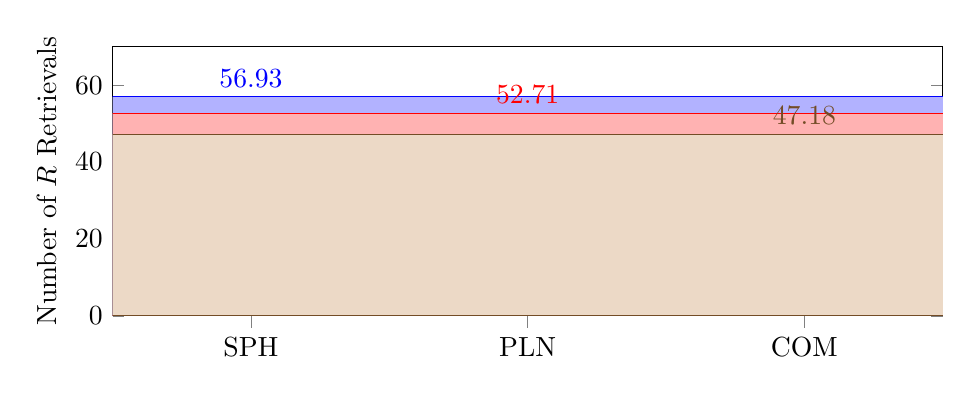
\begin{tikzpicture}
    \begin{axis}[
    ybar,
    width=\linewidth, height=5cm,
    ylabel={Number of $R$ Retrievals}, ylabel near ticks, ymin=0, ymax=70,
    xticklabels={SPH, PLN, COM},
    xtick={1, 2, 3}, xmin=0.5, xmax=3.5, xtick pos=left,
    nodes near coords, nodes near coords align={vertical},
    every axis plot/.append style={
    ybar,
    bar width=40,
    bar shift=0pt,
    fill
    }
    ]
        \addplot coordinates {(1, 56.93)}; % SPH
        \addplot coordinates {(2, 52.71)}; % PLN
        \addplot coordinates {(3, 47.18)};
    \end{axis}
\end{tikzpicture}

%SELECT AVG(QueryCount), IdentificationMethod
%FROM REDUCTION
%WHERE rowid IN (
%    SELECT rowid
%    FROM REDUCTION
%    WHERE (IdentificationMethod LIKE 'Plane' OR IdentificationMethod LIKE 'Sphere')
%    AND ShiftDeviation < 1.0e-3 AND ShiftDeviation > 1.0e-5 AND FalseStars = 0
%    AND QueryCount > 1
%)
%GROUP BY IdentificationMethod

%SELECT AVG(QueryCount)
%FROM REDUCTION
%WHERE rowid IN (
%    SELECT rowid
%    FROM REDUCTION
%    WHERE IdentificationMethod LIKE 'Composite'
%    AND ShiftDeviation < 1.0e-3 AND ShiftDeviation > 1.0e-5 AND FalseStars = 0
%    AND QueryCount > 1
%)
%    \caption{
%    Depicts the average number of database accesses required to obtain a $r$ set for strategies with triangular features given $\sigma \seq \ang{0.0001}$ of Gaussian noise.
%    To characterize the pivoting method itself, we only display instances where $\abs{R}\!\neq\!1$ with the first $b$ selection.
%%    The Spherical Triangle strategy has $1{,}952 / 2{,}000$ runs matching the criteria before, the Planar Triangle
%%    strategy has $1{,}946$ runs, and the Composite Pyramid strategy has $1{,}957$ runs.
%    }\label{fig:rPivot}
%    }
%\end{figure}

%\subsubsection{How expensive is the pivoting process?}
%import numpy as np
%m_1, m_2, s_1, s_2, n_1, n_2 = 52.71, 47.18, 56.794658219949106, 47.01765577951369, 1946, 1957
%z = (m_2 - m_1) / np.sqrt( ((s_1 * s_1) / n_1) + ((s_2 * s_2) / n_2) )
%As seen previously, identification strategies with triangular features have the most instances where $\abs{R} \seq 1$ given an image with no noise.
%~\autoref{fig:rPivot} displays the average number of database accesses for these same strategies where the first image set $b$ selection does not meet the $R$ criterion given an image with Gaussian noise.
%The average number of database accesses is higher in strategies that use the pivoting processes, as opposed to those that do not.
%Given the null hypothesis that the difference between the Planar Triangle strategy's number of database accesses and the Composite Pyramid strategy's number of database accesses is not significant, $z \seq 3.3, p\!<\!0.0001$ is obtained with a two-tailed two sample $Z$ test.
%With the data collected here, we find that the pivoting process results in more database accesses on average.
%This increased number of accesses results in a $6.70\si{ms}$ difference on average between the two.
%
%The pivoting process was only tested with the strategies most frequently meeting the $\abs{R}\seq1 $ criterion.
%An area of interest would be to see the effects of applying this process to strategies with angular features (i.e.\ Angle, Interior Angle, Pyramid).
%These strategies met the criterion less frequently, and would likely benefit from attempting to reduce the $R$ set before deciding to choose another $b$ set.
%
%\subsection{Confidence Check}\label{subsec:identificationStep}
%\subsubsection{How effective is a second confidence check?}
%if __name__ == '__main__':
%from numpy import std, average, sqrt
%from sqlite3 import connect
%from os import environ
%
%conn_1 = connect(environ['HOKU_PROJECT_PATH'] + '/data/lumberjack-all-triad.db')
%conn_2 = connect(environ['HOKU_PROJECT_PATH'] + '/data/lumberjack-pyramid-noverify.db')
%
%name = 'Pyramid'
%
%sample_1 = list(map(lambda b: b.execute("""
%SELECT PercentageCorrect
%FROM IDENTIFICATION
%WHERE ShiftDeviation < 1.0e-7 AND FalseStars = 0
%AND IdentificationMethod LIKE '{}'
%""".format(name)).fetchall(), [conn_1, conn_2]))
%
%sample_2 = list(map(lambda b: b.execute("""
%SELECT PercentageCorrect
%FROM IDENTIFICATION
%WHERE ShiftDeviation < 1.0e-5 AND FalseStars = 0
%AND IdentificationMethod LIKE '{}'
%""".format(name)).fetchall(), [conn_1, conn_2]))
%
%sample_3 = list(map(lambda b: b.execute("""
%SELECT PercentageCorrect
%FROM IDENTIFICATION
%WHERE ShiftDeviation < 1.0e-2 AND ShiftDeviation > 1.0e-4 AND FalseStars = 0
%AND IdentificationMethod LIKE '{}'
%""".format(name)).fetchall(), [conn_1, conn_2]))
%
%flatten = lambda a: [b[0] for b in a]
%for i, sample in enumerate([sample_1, sample_2, sample_3]):
%n_1, n_2 = 2000, 2000
%m_1, m_2 = average(flatten(sample[0])), average(flatten(sample[1]))
%s_1, s_2 = std(flatten(sample[0])), std(flatten(sample[1]))
%print('Z Score of {}: {}'.format(i, (m_2 - m_1) / sqrt( ((s_1 * s_1) / n_1) + ((s_2 * s_2) / n_2) )))

%import numpy as np
%print(np.average( [6.97725 - 3.00525, 6.9615 - 3.005, 398.0655 -  ))
%In~\autoref{fig:verify}, the accuracy of the map produced by the Pyramid and Composite Pyramid strategies are displayed with and without the second confidence check for varying levels of Gaussian noise.
%In~\autoref{algorithm:pyramidIdentification}, this refers to the \Call{ConfidenceCheck}{} function.
%Without noise, the Pyramid strategy without its second confidence check is 4.33\% less accurate than the Pyramid strategy with its original configuration on average.
%This behavior is consistently seen for Gaussian noise of $\sigma\seq\ang{0.000001}$ \& $\sigma\seq\ang{0.001}$, and can be attributed to the more frequent rejection of incorrect maps with $R$ sets that have met the criterion.
%In the $\sigma\seq\ang{0.001}$ case, there exists a difference of 389.95 accesses between both variations of the Pyramid and a 15\% mapping accuracy difference in favor of the strategy with the original configuration.
%Given the null hypotheses that the difference between both variations of the Pyramid strategy are different for each level of noise, $z_0 \seq 15.87, z_{0.000001} \seq 16.04, z_{0.001} \seq 12.14$ (all $p\!<\!0.0001$) is obtained with two-tailed two sample $Z$ tests.
%The verification step increases the accuracy of the Pyramid strategy.
%
%\begin{figure}
%    \centering{
%        \begin{tikzpicture}
    \begin{axis}[
    ybar,
    width=\linewidth, height=5cm,
    ylabel={$a(h, b, r)$}, ylabel near ticks, ymin=0, ymax=1.3,
    xtick={1, 2, 3}, xticklabels={$\ang{0}$, $\ang{0.000001}$, $\ang{0.001}$},
    xlabel={$\sigma$ of Noise (degrees)}, xmin=0.5, xmax=3.5, xtick pos=left,
    nodes near coords, every node near coord/.append style={rotate=90, anchor=west},
    legend style={at={(0.5,-0.35)}, anchor=north,legend columns=-1},
    bar width=7
    ]
        \addplot coordinates {(1, 0.999416666666667) (2, 0.999222222222222) (3, 0.354333333333333)};
        \addplot coordinates {(1, 0.956083333333329) (2, 0.954444444444449) (3, 0.203166666666665)};
        \addplot coordinates {(1, 1.0) (2, 1.0) (3, 0.0)};
        \addplot coordinates {(1, 1.0) (2, 0.999833333333333) (3, 0.346333333333333)};
        \legend{PYR, PYR-N, COM, COM-N}
    \end{axis}
\end{tikzpicture}
%        \caption{
%        Depicts the frequency of correct maps (\texttt{ACC}) formed with and without the second confidence step (\Call{ConfidenceCheck}{}) of both the Pyramid and Composite Pyramid strategies.
%        There exists $2{,}000$ runs for each identification strategy, with a database access limit (i.e.\ number of times the database is searched) of 500.
%        The `-N' suffix indicates the strategy bypasses \Call{ConfidenceCheck}{}.
%%        PYR corresponds to the Pyramid method with the verification step, PYR-N corresponds to the Pyramid method
%%        without the verification step, COM corresponds to the Composite Pyramid method with the verification step,
%%        and COM-N corresponds to the Composite Pyramid method without the verification step.
%        }\label{fig:verify}
%    }
%\end{figure}
%
%\begin{figure*} % HAD TO MOVE THIS GUY TOO...
%    \centering{
%    \begin{subfigure}[b]{0.48\linewidth}
%        \begin{tikzpicture}
    \begin{axis}[
    ybar,
    width=\linewidth, height=5cm,
    ylabel={$t \ (\si{ms})$}, ylabel near ticks, ymin=10, ymax=100000,
    xtick={1, 2, 3}, xticklabels={$\ang{0}$, $\ang{0.0001}$, $\ang{0.01}$},
    xlabel={$\sigma$ (degrees)}, xmin=0.5, xmax=3.5, xtick pos=left, point meta=rawy,
    nodes near coords, every node near coord/.append style={rotate=90, anchor=west,
    /pgf/number format/.cd,fixed,precision=6},
    legend style={at={(0.5,-0.35)}, anchor=north,legend columns=-1},
    bar width=7, ymode=log, log origin=infty, max space between ticks=20
    ]
        \addplot coordinates {(1, 1197.43) (2, 1349.07) (3, 6509.00)};
        \addplot coordinates {(1, 160.68) (2, 161.80) (3, 872.22)};
        \addplot coordinates {(1, 323.94) (2, 339.23) (3, 392.29)};
        \addplot coordinates {(1, 324.35) (2, 328.85) (3, 352.24)};
        \addplot coordinates {(1, 170.79) (2, 171.53) (3, 364.04)};
        \addplot coordinates {(1, 405.53) (2, 1545.45) (3, 362.30)};
        \legend{ANG, INT, SPH, PLN, PYR, COM}
    \end{axis}
\end{tikzpicture}
%    \end{subfigure}
%    \begin{subfigure}[b]{0.48\linewidth}
%        %if __name__ == '__main__':
%    from numpy import std, average, sqrt, polyfit, log
%    from sqlite3 import connect
%    from os import environ
%
%    conn_1 = connect(environ['HOKU_PROJECT_PATH'] + '/data/lumberjack-all-triad.db')
%    cur = conn_1.cursor()
%
%    # 1,   2,      3,      4,      5,     6,    7,   8
%    # 0.0, 1.0e-6, 1.0e-5, 0.0001, 0.001, 0.01, 0.1, 1.0
%
%    for d in [[1, 2, 3, 4, 5, 6, 7, 8], [0.0, 1.0e-6, 1.0e-5, 0.0001, 0.001, 0.01, 0.1, 1.0]]:
%        t = polyfit(log(d[3:]), [0.9725, 0.386, 0.0035, 0.0, 0.0], 1)
%        print('Angle: {}*ln(x) + {}'.format(t[0], t[1]))
%
%        t = polyfit(log(d[4:]), [0.9885, 0.7055, 0.033, 0.00383333333333333], 1)
%        print('Dot: {}*ln(x) + {}'.format(t[0], t[1]))
%
%        t = polyfit(log(d[2:]), [0.9715, 0.8135, 0.259, 0.0253333333333333, 0.0095, 0.00716666666666667], 1)
%        print('Sphere: {}*ln(x) + {}'.format(t[0], t[1]))
%
%        t = polyfit(log(d[2:]), [0.9865, 0.8615, 0.332166666666667, 0.0245, 0.0095, 0.00483333333333333], 1)
%        print('Plane: {}*ln(x) + {}'.format(t[0], t[1]))
%
%        t = polyfit(log(d[3:]), [0.999333333333334, 0.354333333333333, 0.0, 0.0, 0.0], 1)
%        print('Pyramid: {}*ln(x) + {}'.format(t[0], t[1]))
%
%        t = polyfit(log(d[1:]), [1.0, 0.65, 0.0035, 0.0, 0.0, 0.0, 0.0], 1)
%        print('Composite: {}*ln(x) + {}'.format(t[0], t[1])), print()

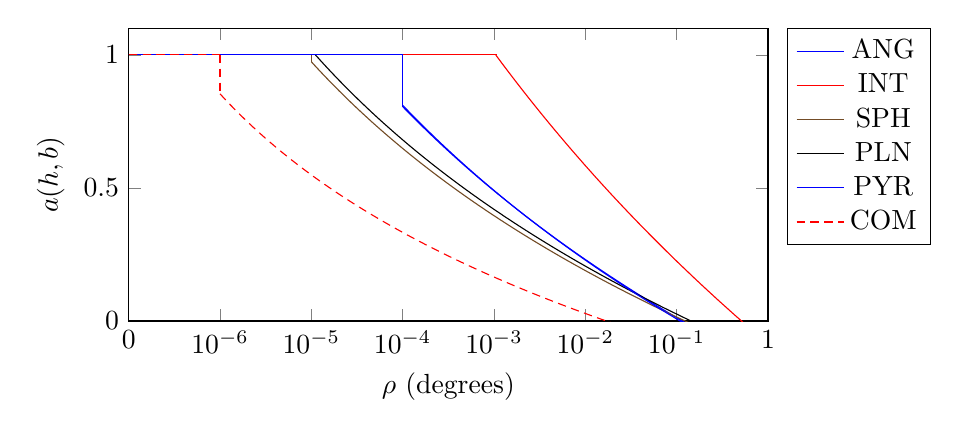
\begin{tikzpicture}
    \begin{axis}[
    width=0.8\linewidth, height=5.3cm,
    ylabel={$a(h, b)$}, ymin=0, ymax=1.1,
    xlabel={$\rho$ (degrees)}, xmin=1, xmax=8,
    xtick={1, 2, 3, 4, 5, 6, 7, 8},
    xticklabels={$0$, $10^{-6}$, $10^{-5}$, $10^{-4}$, $10^{-3}$, $10^{-2}$, $10^{-1}$, $1$},
    samples=100, no markers, legend pos=outer north east, enlargelimits=false
    ]
        \addplot +[domain=1:4, forget plot]{1};
        \addplot +[forget plot] coordinates {(4, 1) (4, 0.8055384229041530)};
        \addplot +[domain=4:8]{-1.416887591459587*ln(x) + 2.7697617012853217};
        \addlegendentry{ANG}

        \addplot +[domain=1:5.03, forget plot]{1};
%        \addplot +[forget plot] coordinates {(5, 1) (5, 1)};
        \addplot +[domain=5.02:8]{-2.3292306442173216*ln(x) + 4.757244753386215};
        \addlegendentry{INT}

        \addplot +[domain=1:3, forget plot]{1};
        \addplot +[forget plot] coordinates {(3, 1) (3, 0.9738787471803161)};
        \addplot +[domain=3:8]{-1.1317828984553227*ln(x) + 2.217269347527745};
        \addlegendentry{SPH}

        \addplot +[domain=1:3, forget plot]{1};
%        \addplot +[forget plot] coordinates {(3, 1) (3, )};
        \addplot +[domain=3.04:8]{-1.1696544292494204*ln(x) + 2.301996347627258};
        \addlegendentry{PLN}

        \addplot +[domain=1:4, forget plot]{1};
        \addplot +[forget plot] coordinates {(4, 1) (4, 0.8105837347641904)};
        \addplot +[domain=4:8]{-1.4347255837709008*ln(x) + 2.7995357213002334};
        \addlegendentry{PYR}

        \addplot +[domain=1:2, forget plot]{1};
        \addplot +[forget plot] coordinates {(2, 1) (2, 0.8533960244900531)};
        \addplot +[domain=2:8]{-0.7510156659772902*ln(x) + 1.3739604159185614};
        \addlegendentry{COM}
    \end{axis}
\end{tikzpicture}
%    \end{subfigure}
%    \caption{
%    Both plots represent a statistic about the resulting map $h$ produced by each identification strategy given some image with varying Gaussian noise.
%    There exists $2{,}000$ runs for each identification strategy, with the number of database accesses limited to 500.
%    The left plot depicts the average time to obtain $h$, and the right plot depicts the trend line $\texttt{ACC} = c \cdot \mathit{\ln}\left( \sigma \right) + d$.
%    }\label{fig:gaussianNoise}
%    }
%\end{figure*}

%The response to Gaussian noise for the Composite Pyramid begins at $\sigma\seq\ang{0.001}$, with a 34.6\% difference between the two variants in favor of the strategy without the second confidence check.
%Unlike the second confidence check in the Pyramid strategy, this filter appears to be too aggressive for the Composite Pyramid strategy.
%The variant without the second confidence check has an average of 193.93 database accesses at $\sigma\seq\ang{0.001}$.
%Without the second confidence check, the Composite Pyramid strategy only had an average of 8.114 database accesses, suggesting that the $\abs{R} \seq 1$ criterion and the \Call{DMT}{} process are sufficient enough for rejecting incorrect $R$ sets and maps.
%
%\subsection{End to End}\label{subsec:endToEndEvaluation}
%\subsubsection{Which strategy is the fastest given no noise?}
%In~\autoref{fig:gaussianNoise}, the left plot depicts the end to end running time of each identification strategy given varying degrees of Gaussian noise.
%In the no noise case, the Angle strategy is the slowest identification strategy on average.
%The next slowest strategy is the Composite Pyramid strategy, a factor of 2.95 times faster than the Angle strategy.
%Recall that the Angle strategy had the fastest candidate retrieval, but the largest $\abs{R}$.
%On average, it takes 69.85 database accesses to obtain a mapping and 68.10 database accesses to meet the $\abs{R} \seq 1$ criterion.
%This suggests that the Angle strategy's long running time stems from the $\abs{R} \seq 1$ criterion and not the \Call{DMT}{} process.

%import numpy as np
%m_1, m_2, s_1, s_2, n_1, n_2 = 160.675, 170.7905, 0.53808, 0.52922, 2000, 2000
%z = (m_2 - m_1) / np.sqrt( ((s_1 * s_1) / n_1) + ((s_2 * s_2) / n_2) )
%The fastest strategy in the no noise case appears to be the Interior Angle strategy, with the second fastest strategy running 10.11 \si{ms} slower.
%There exists $0 / 2{,}000$ runs where the Interior Angle strategy runs above the Pyramid strategy's average running time ($170.79$ $\si{ms}$) and the Interior Angle strategy has the fastest recorded identification run of $135\si{ms}$.
%The Interior Angle strategy is the fastest identification strategy given no noise.

%\subsubsection{Which strategy is the fastest given varying levels of Gaussian noise?}
%As Gaussian noise is increased from $\sigma\seq\ang{0}$ to $\sigma\seq\ang{0.01}$, the Angle strategy experiences the largest response of $5{,}311.57$ additional $\si{ms}$.
%The next slowest strategy in the noise of $\rho\seq\ang{0.01}$ case is the Interior Angle strategy, a factor of 7.46 times faster than the Angle strategy.
%On average, the Angle strategy takes 399.66 database accesses to obtain a mapping and only 36.72 accesses to obtain $r$ here.
%In the no noise case, this strategy's long running time can attributed to the aggressive $R$ criterion.
%Given Gaussian noise, the \Call{DMT}{} process plays a larger role with the Angle strategy and returns to $b$ decision process more often.
%
%The Composite Pyramid strategy shows an interesting runtime response to this type of noise, running $1{,}139.92\si{ms}$ longer given $\ang{0.0001}$ of noise from no noise but $1{,}183.15\si{ms}$ shorter from $\ang{0.0001}$ of noise to $\ang{0.01}$.
%The Pyramid strategy is observed to have this same running time response against noise at $\sigma\seq\ang{0.001}$ (not depicted).
%The most probable explanation lies in how far each run travels from the $b$ decision step.
%At $\sigma\seq\ang{0.0001}$, the Composite Pyramid has gone through the $\abs{R} \seq 1$ criterion and is likely choosing another $b$ set after the verification step.
%At $\sigma\seq\ang{0.01}$ the strategy is not passing the same criterion, avoiding the verification step.

%if __name__ == '__main__':
%from numpy import std, average, sqrt
%from sqlite3 import connect
%from os import environ
%
%conn_1 = connect(environ['HOKU_PROJECT_PATH'] + '/data/lumberjack-all-triad.db')
%conn_2 = connect(environ['HOKU_PROJECT_PATH'] + '/data/lumberjack-pyramid-noverify.db')
%
%sample_1 = conn_1.execute("""
%SELECT TimeToResult
%FROM IDENTIFICATION
%WHERE ShiftDeviation > 1.0e-7 AND FalseStars = 0
%AND IdentificationMethod LIKE 'Plane'
%""").fetchall()
%
%sample_2 = conn_1.execute("""
%SELECT TimeToResult
%FROM IDENTIFICATION
%WHERE ShiftDeviation > 1.0e-7 AND FalseStars = 0
%AND IdentificationMethod LIKE 'Pyramid'
%""").fetchall()
%
%flatten = lambda a: [b[0] for b in a]
%n_1, n_2 = 12000, 12000
%m_1, m_2 = average(flatten(sample_1)), average(flatten(sample_2))
%s_1, s_2 = std(flatten(sample_1)), std(flatten(sample_2))
%print('Z Score of: {}'.format((m_2 - m_1) / sqrt( ((s_1 * s_1) / n_1) + ((s_2 * s_2) / n_2) )))
%The fastest strategy on average given images with Gaussian noise $\sigma \in \set{10^{-1}, 10^{-2}, \ldots, 10^{-6}}$ is the Pyramid strategy at $288.44$ $\si{ms}$ (of 12,000 runs).
%%\begin{equation}\label{eq:sigmasTested}
%%    \rho \in \set{10^{-1}, 10^{-2}, \ldots, 10^{-6}}
%%\end{equation}
%The second fastest strategy given the same noise set is the Planar Triangle strategy at $341.16\si{ms}$.
%Given the null hypothesis that the difference between both averages is not significant, $z \seq 24.32, p\!<\!0.0001$ is found with a two-tailed two sample $Z$ test.
%With the data collected here, the Pyramid strategy is the fastest strategy given varying amounts of Gaussian noise.
%
%\begin{figure*}
%    \centering{
%    \begin{subfigure}[b]{0.48\linewidth}
%        \begin{tikzpicture}
    \begin{axis}[
    ybar,
    width=\linewidth, height=5cm,
    ylabel={$t \ (\si{ms})$}, ylabel near ticks, ymin=10, ymax=100000,
    xtick={1, 2, 3}, xticklabels={0, 6, 12},
    xlabel={$\omega$}, xmin=0.5, xmax=3.5, xtick pos=left, point meta=rawy,
    nodes near coords, every node near coord/.append style={rotate=90, anchor=west,
    /pgf/number format/.cd,fixed,precision=2},
    legend style={at={(0.5,-0.35)}, anchor=north,legend columns=-1},
    bar width=7, ymode=log, log origin=infty, max space between ticks=20
    ]
        \addplot coordinates {(1, 1197.43) (2, 1737.94) (3, 2431.58)};
        \addplot coordinates {(1, 160.68) (2, 209.36) (3, 280.54)};
        \addplot coordinates {(1, 323.94) (2, 355.54) (3, 386.20)};
        \addplot coordinates {(1, 324.35) (2, 350.60) (3, 390.41)};
        \addplot coordinates {(1, 170.79) (2, 183.71) (3, 195.53)};
        \addplot coordinates {(1, 405.53) (2, 685.07) (3, 972.04)};
        \legend{ANG, DOT, SPH, PLN, PYR, COM}
    \end{axis}
\end{tikzpicture}
%    \end{subfigure}
%    \begin{subfigure}[b]{0.48\linewidth}
%        \begin{tikzpicture}
    \begin{axis}[
    ybar,
    width=\linewidth, height=5cm,
    ylabel={Accuracy of Map, \texttt{ACC}}, ylabel near ticks, ymin=0, ymax=1.4,
    xtick={1, 2, 3}, xticklabels={0, 6, 12},
    xlabel={$\omega$}, xmin=0.5, xmax=3.5, xtick pos=left,
    nodes near coords, every node near coord/.append style={rotate=90, anchor=west,
    /pgf/number format/.cd,fixed,precision=4},
    legend style={at={(0.5,-0.35)}, anchor=north,legend columns=-1},
    bar width=7
    ]
        \addplot coordinates {(1, 0.977) (2, 0.979) (3, 0.960)};
        \addplot coordinates {(1, 1.0) (2, 0.982) (3, 0.965)};
        \addplot coordinates {(1, 1.0) (2, 0.840) (3, 0.696)};
        \addplot coordinates {(1, 1.0) (2, 0.845) (3, 0.703)};
        \addplot coordinates {(1, 0.999) (2, 0.999) (3, 0.995)};
        \addplot coordinates {(1, 1.0) (2, 0.994) (3, 0.973)};
        \legend{ANG, INT, SPH, PLN, PYR, COM}
    \end{axis}
\end{tikzpicture}
%    \end{subfigure}
%    \caption{
%    Both plots represent a statistic about the resulting map $h$ produced by each identification strategy given some image with varying amounts of spikes $\omega$.
%    There exists $2{,}000$ runs for each identification strategy, with the number of database accesses limited to 500.
%    The left plot depicts the average time to obtain a map $h$, and the right plot depicts the average accuracy of the produced $h$.
%    }\label{fig:falseNoise}
%    }
%\end{figure*}

%\subsubsection{Which strategy has the slowest growing map accuracy response to increasing noise?}
%The selection of the retrieval $\epsilon$ parameters plays a significant role in accuracy of each strategy given images with Gaussian noise.
%For strategies that search the database using on the $\theta$ feature (Angle, Interior Angle, Pyramid), the $\epsilon$ parameter serves as a rough upper bound for the amount of Gaussian noise tolerated.
%In~\autoref{fig:gaussianNoise}, the plot on the right depicts the accuracy of resulting injection of each method for
%varying levels of Gaussian noise.
%When the level of noise is equal to the Angle and Pyramid $\epsilon_\theta$ parameter ($\ang{0.0001}$), both strategies have an average $h$ accuracy of $98.59\!\pm\!1.34\%$.
%When Gaussian noise is increased to $\ang{0.001}$, both strategies drop to $47.02\!\pm\!1.58\%$.

%For strategies with features that are not angular (Spherical Triangle, Planar Triangle, Composite Pyramid), characterizing the effect of Gaussian noise becomes more difficult.
%These strategies have the parameters $\epsilon_a \seq 3\cdot 10^{-9}$ and $\epsilon_\tau \seq 3\cdot10^{-9}$, showing an initial accuracy response to noise at $\ang{0.00001}$.
%The Interior Angle method has the largest query $\sigma$ parameters, and only experiences a response to noise at
%$\ang{0.01}$.
%Given the current set of query $\sigma$, the Interior Angle is the most accurate method on average.

%Ranking each strategy based on their $h$ accuracy is not particularly insightful here given the heavy dependence on $\epsilon$ parameters, so instead we analyze the rate of change involved with varying levels of noise.
%The right plot in~\autoref{fig:gaussianNoise} depicts the trend line for all strategies where $h$ accuracy (denoted as \texttt{ACC}) is displayed against the amount of Gaussian noise.
%It has been observed that the accuracy of each strategy remains near 100\% until it decreases exponentially to zero:
%\begin{equation}
%    \texttt{ACC} =
%    \begin{cases}
%        0 & \sigma < 0 \\
%        1 & 0 \leq \sigma < \hat{\sigma} \\
%        c \cdot \ln(\sigma) + d & \sigma \geq \hat{\sigma}
%    \end{cases}
%\end{equation}
%Each line was fit to the piecewise equation above ($c\cdot \ln(\sigma) + d$ term with least squares), where $c$ and $d$ are the parameters found with the regression, $\texttt{ACC}$ is the accuracy of the map $h$, and $\hat{\sigma}$ is the point where $\texttt{ACC}$ is observed to dip below 95\%.
%The accuracy acceleration varies across strategies through the value of $c$:
%\begin{equation}
%    \frac{d^{2}\texttt{ACC}}{d\sigma^2} = \frac{-c}{\sigma^2}, \ \ \sigma \geq \hat{\sigma}
%\end{equation}
%A larger $c$ suggests that a change in retrieval $\epsilon$ or Gaussian noise will not affect the accuracy of the strategy as much as a strategy with a larger $c$.
%The strategy with the largest acceleration toward $0\%$ \texttt{ACC} is the Interior Angle strategy ($c \seq -0.15749$).
%The Spherical Triangle strategy has the slowest growing \texttt{ACC} response to increasing noise ($c \seq -0.09266$).
%
%\subsubsection{Which strategy is the fastest given varying amounts of false points?}
%In~\autoref{fig:falseNoise}, the plot on the left depicts the end to end running time of each strategy given varying amounts of spikes (i.e.\ false points).
%As the number of spikes increases from 0 to 12, the Angle strategy again experiences the largest response of $1{,}234.15$ $\si{ms}$.
%The next fastest strategy is the Composite Pyramid strategy, a factor of 2.50 times faster than the Angle strategy.
%The difference between the 1st and 2nd slowest strategies is 2.98 times less than the Gaussian noise case.
%On average, it takes 114.23 database accesses to obtain a map and only 54.85 accesses to obtain $r$.
%Relative to the Gaussian noise comparison, \Call{DMT}{} and $\abs{R} \seq 1$ criterion play a more equal role in the decision to choose a new $b$ set.

%if __name__ == '__main__':
%from numpy import std, average, sqrt
%from sqlite3 import connect
%from os import environ
%
%conn_1 = connect(environ['HOKU_PROJECT_PATH'] + '/data/lumberjack-all-triad.db')
%conn_2 = connect(environ['HOKU_PROJECT_PATH'] + '/data/lumberjack-pyramid-noverify.db')
%
%sample_1 = conn_1.execute("""
%SELECT TimeToResult
%FROM IDENTIFICATION
%WHERE FalseStars > 0
%AND IdentificationMethod LIKE 'Pyramid'
%""").fetchall()
%
%sample_2 = conn_1.execute("""
%SELECT TimeToResult
%FROM IDENTIFICATION
%WHERE FalseStars > 0
%AND IdentificationMethod LIKE 'Dot'
%""").fetchall()
%
%flatten = lambda a: [b[0] for b in a]
%n_1, n_2 = 8000, 8000
%m_1, m_2 = average(flatten(sample_1)), average(flatten(sample_2))
%s_1, s_2 = std(flatten(sample_1)), std(flatten(sample_2))
%print('Z Score of: {}'.format((m_2 - m_1) / sqrt( ((s_1 * s_1) / n_1) + ((s_2 * s_2) / n_2) )))
%The fastest strategy on average given images with spikes is the Pyramid strategy at $186.22\si{ms}$.
%The images given to each strategy contained $\omega$ spikes, where $\omega \in \set{ 3, 6, 9, 12 }$.
%The second fastest strategy given the same noise set is the Interior Angle strategy at $228.37\si{ms}$.
%Given the null hypothesis that the difference between both averages is not significant, $z \seq 28.47, p\!<\!0.0001$ is
%found with a two-tailed two sample $Z$ test.
%The Pyramid strategy is the fastest strategy given varying amounts of spikes.
%The process for choosing distinct image subsets is shown to be the fastest approach to finding a map that meets the Pyramid's confidence checks.

%if __name__ == '__main__':
%from numpy import std, average, sqrt, polyfit, log
%from sqlite3 import connect
%from os import environ
%
%conn_1 = connect(environ['HOKU_PROJECT_PATH'] + '/data/lumberjack-all-triad.db')
%cur = conn_1.cursor()
%
%for name in ['Angle', 'Dot', 'Sphere', 'Plane', 'Pyramid', 'Composite']:
%sample_1 = list(map(lambda a: a[0], cur.execute("""
%SELECT AVG(TimeToResult)
%FROM IDENTIFICATION
%WHERE FalseStars > 0
%AND IdentificationMethod LIKE ?
%GROUP BY FalseStars
%ORDER BY FalseStars
%""", (name, )).fetchall()))
%
%t = polyfit([3, 6, 9, 12], sample_1, 1)
%print('{name}: {t_0}*x + {t_1}'.format(name=name, t_0=round(t[0], 5), t_1=round(t[1], 5)))
%Each strategy exhibits a linear increase to runtime as additional spikes are added.
%To characterize each strategy's runtime as a function of false points, each strategy's runtime was fit to a linear equation using least squares:
%\begin{equation}
%    t = c\cdot\omega + d
%\end{equation}
%where $c$ and $d$ are the parameters found with the regression and $t$ is the end to end running time of the strategy.
%A smaller $\abs{c}$ suggests that the number of spikes will affect the end to end runtime than that of a strategy with a larger $\abs{c}$.
%The strategy with the largest $\abs{c}$ is the Angle strategy with $c \seq -414.559$.
%The strategy with the smallest $\abs{c}$ term is the Pyramid strategy with $c \seq -6.766$.
%The Pyramid strategy is the fastest given varying amounts of false points, having a runtime that is also the least responsive to increasing spikes.

%\subsubsection{Which strategy is the most accurate given varying amounts of false points?}
%if __name__ == '__main__':
%from numpy import std, average, sqrt
%from sqlite3 import connect
%from os import environ
%
%conn_1 = connect(environ['HOKU_PROJECT_PATH'] + '/data/lumberjack-all-triad.db')
%conn_2 = connect(environ['HOKU_PROJECT_PATH'] + '/data/lumberjack-pyramid-noverify.db')
%
%sample_1 = conn_1.execute("""
%SELECT PercentageCorrect
%FROM IDENTIFICATION
%WHERE FalseStars = 12
%AND (IdentificationMethod LIKE 'Plane' OR IdentificationMethod LIKE 'Sphere')
%""").fetchall()
%
%sample_2 = conn_1.execute("""
%SELECT PercentageCorrect
%FROM REDUCTION
%WHERE FalseStars = 12
%AND (IdentificationMethod LIKE 'Plane' OR IdentificationMethod LIKE 'Sphere')
%""").fetchall()
%
%flatten = lambda a: [b[0] for b in a]
%n_1, n_2 = 2000, 2000
%m_1, m_2 = average(flatten(sample_1)), average(flatten(sample_2))
%s_1, s_2 = std(flatten(sample_1)), std(flatten(sample_2))
%print('Z Score of: {}'.format((m_2 - m_1) / sqrt( ((s_1 * s_1) / n_1) + ((s_2 * s_2) / n_2) )))
%In~\autoref{fig:falseNoise}, the plot on the right depicts the average accuracy of each mapping given varying amounts of spikes.
%As the number of false points is increased from $\omega \seq 0$ to $\omega \seq 12$, the strategies that experience the largest $h$ accuracy response are the Spherical Triangle strategy ($30.42\%$ average decrease) and the Planar Triangle strategy ($29.68\%$ average decrease).
%The average accuracy of the candidate selection is a few percent less than the average accuracy of $h$ here ($0.53\!\pm\!1.78\%$ for both strategies).
%Given the null hypothesis that the difference between the accuracy of the $h$ map and the accuracy of the candidate selection is not significant, $z \seq 0.37, p \seq 0.71$ was found with a two-tailed two sample $Z$ test.
%There does not exist enough data to reject this hypothesis with $\alpha \seq 0.01$.
%This suggests that the \Call{DMT}{} process is neither helpful or detrimental to the end to end accuracy of these strategies.
%
%Ruling out the \Call{DMT}{} process, the most likely source of error for the triangle strategies is their decision of different $b$ sets.
%If a false point exists as $b[1]$ in $b$, the triangle strategies will have to iterate through $n^2$ combinations and $n - 3$ pivots at most to choose another point that is not the spike.
%The Angle strategy only has to wait $n$ additional combinations at most if a false point exists in $b$.
%The Interior Angle strategy is able to get around the spike persistence problem by choosing $b$ sets based on their $\theta$ proximity to the central point.
%The Pyramid and Composite Pyramid strategies have their $b$ decision process designed for this situation, increasing the average turnover of all points in the $b$ set.
%
%The Pyramid strategy has the most accurate map $h$ on average given images with all different $\omega$ at $99.84\!\pm\!3.53\%$.
%The second most accurate strategy is the Composite Pyramid strategy at $99.19\!\pm\!8.95\%$.
%Given the null hypothesis that the difference between the mapping accuracies of both strategies is not significant, $z \seq 3.02, p \seq 0.003$ with a two-tailed two sample $Z$ test.
%At $\alpha \seq 0.01$, our hypothesis does not hold true.
%The Pyramid strategy is the most accurate under varying amounts of spikes.
